%compile then compile with biber (for the biblio) then recompile
\documentclass[12pt]{article}

\usepackage{a4wide} % increase the typeset area
\usepackage{bm}
\usepackage{amsmath,amssymb}
\usepackage{enumitem}
\usepackage{graphicx}
\usepackage{color}
\usepackage{float} %to place figure H
\usepackage{multirow} %multirow for table
%\usepackage[super]{natbib} %exponant biblio
\usepackage{fourier} %for danger sign
\usepackage{chngcntr}
\usepackage{pifont} %for more symbol in enumerate

% Useful packages for table

\usepackage{array,multirow,makecell}
\usepackage[linesnumbered]{algorithm2e}
\usepackage[table]{xcolor}
\setcellgapes{1pt}
\makegapedcells
\newcolumntype{R}[1]{>{\raggedleft\arraybackslash }b{#1}}
\newcolumntype{L}[1]{>{\raggedright\arraybackslash }b{#1}}
\newcolumntype{C}[1]{>{\centering\arraybackslash }b{#1}}



%hyperref
\usepackage[colorlinks]{hyperref}
\hypersetup{
	colorlinks=true,
	linkcolor=blue,
	filecolor=magenta,      
	urlcolor=blue,
	citecolor=blue
}

% captions
\usepackage{caption}
\newcommand{\vect}[1]{\hat{\boldsymbol{#1}}}
\usepackage{subcaption}
\counterwithin{figure}{section}
\makeatletter
\usepackage[labelformat=simple]{subcaption}
\newcommand\captionsubfigure{%
	\renewcommand\p@subfigure{}
	\renewcommand\thesubfigure{\thefigure.\alph{subfigure}}
}
\makeatother

%to make the appendix
\usepackage{appendix}

%code
\usepackage{listings}
\definecolor{backcolor}{RGB}{240, 240, 240}
\lstdefinestyle{bash}{
	commentstyle=\color{green},
	morecomment=[l][\color{magenta}]{\#},
	backgroundcolor=\color{backcolor},  
	breakatwhitespace=false,
	keepspaces=true,                        
	showspaces=false,                
	showstringspaces=false,
	showtabs=false,                  
	tabsize=1    
}

%for footnote
\usepackage[symbol]{footmisc}
\renewcommand{\thefootnote}{\fnsymbol{footnote}}

%bibliography (with section)
\usepackage[backend=biber,style=numeric,sorting=nyt]{biblatex}
\addbibresource{biblio_ref.bib}
\addbibresource{biblio_doc.bib}


% Titlepage
\newcommand{\reporttitle}{Internship Report : Parareal method and data assimilation for PDEs with Feel++}
\newcommand{\reportauthorOne}{Melissa Aydogdu}
\newcommand{\reportauthorTwo}{Frédérique Lecourtier}
\newcommand{\reportsupervisorOne}{Christophe Prudhomme}
\newcommand{\reportsupervisorTwo}{Luca Berti}
\newcommand{\reporttype}{Coursework}

\begin{document}
	\nocite{*}
	
	\begin{titlepage}

\newcommand{\HRule}{\rule{\linewidth}{0.5mm}} % Defines a new command for the horizontal lines, change thickness here

\begin{center} % Center remainder of the page


\includegraphics[width = 0.5\linewidth]{images/logo-cemosis.pdf}\\[1.5cm] 

\textsc{\Large University of Strasbourg}\\[0.5cm] 
\textsc{\large Master CSMI}\\[0.95cm] 

%----------------------------------------------------------------------------------------
%	TITLE SECTION
%----------------------------------------------------------------------------------------

\HRule \\[0.4cm]
{ \huge \bfseries \reporttitle}\\ % Title of your document
\HRule \\[1.5cm]
\end{center}
%----------------------------------------------------------------------------------------
%	AUTHOR SECTION
%----------------------------------------------------------------------------------------

%\begin{minipage}{0.4\hsize}
\begin{flushleft} \large
	\begin{minipage}{0.4\hsize}
		\textit{Authors:}\\
		\reportauthorOne\\
		\reportauthorTwo
	\end{minipage} \hfill 
	\begin{minipage}{0.4\hsize}
		\textit{Supervisors:}\\
		\reportsupervisorOne\\
		\reportsupervisorTwo
	\end{minipage}
\end{flushleft}
\vspace{4cm}
\makeatletter
Date: \@date 

\vfill % Fill the rest of the page with whitespace



\makeatother


\end{titlepage}


	
	\tableofcontents
	
	\newpage
	\section{Introduction}
	
	\noindent This internship is the continuation of a project realised in th platform Cemosis . During the project the main goals were to implement a parallel-in-time resolution method for the Lorenz system, to realize the data assimilation using the EnKF method using a function already implemented in the library Filterpy. For this we also had to implement several methods to solve numerically the Lorenz system (like RK4). During the project, all these methods were implemented or used in Python.
	
	\subsection{Presentation of Cemosis}
	\label{cemosis}
	
	This project is managed by Cemosis which is the "Centre de Modélisation et de Simulation de Strasbourg" (Strasbourg Modeling and Simulation Center). Cemosis is hosted by the Institute of Advanced Mathematical Research (IRMA) and was created in January 2013. 
	Cemosis work is focused on the numarical simulation and mathematical modeling of different phenomena. They use and develop tools in the fields of:
	
	\begin{enumerate}[label=\textbullet]
		\item \textbf{MSO} - Modeling Simulation and Optimization
		\item \textbf{DS} -	Data Science, Big Data, Smart Data
		\item \textbf{HPC} - High Performance Computing, Parallel Computing, Cloud Computing
		\item \textbf{SI} - Signal and Image processing
	\end{enumerate}
	\noindent They work with researchers and engineers of other research centers and companies.
	
	\noindent For more informations, refer to the \href{http://www.cemosis.fr/}{cemosis website}. 
	\subsection{Context}
	\noindent Cemosis relies currently on the team Modeling and Control of the IRMA and is developing competences and projects in the energy sector of buildings. Nowadays it is important to reduce the energy consumption of buildings in order to move to a more ecologic and economic lifestyle. For this we need to know how to simulate and model buildings using fast simulation methods such as parallel calculation and data integration because our models used to simulate buildings are never perfect, and even less in the case of existing buildings where we have little information. In fact, in order to perform simulations over long periods, such as a year, we would also have to take into consideration phenomena such as radiative exchanges and convective effects, which therefore require a PDE model if we want a spatial discretization.
	\begin{figure}[H]       
	\begin{minipage}[t]{0.48\linewidth}
		\centering
		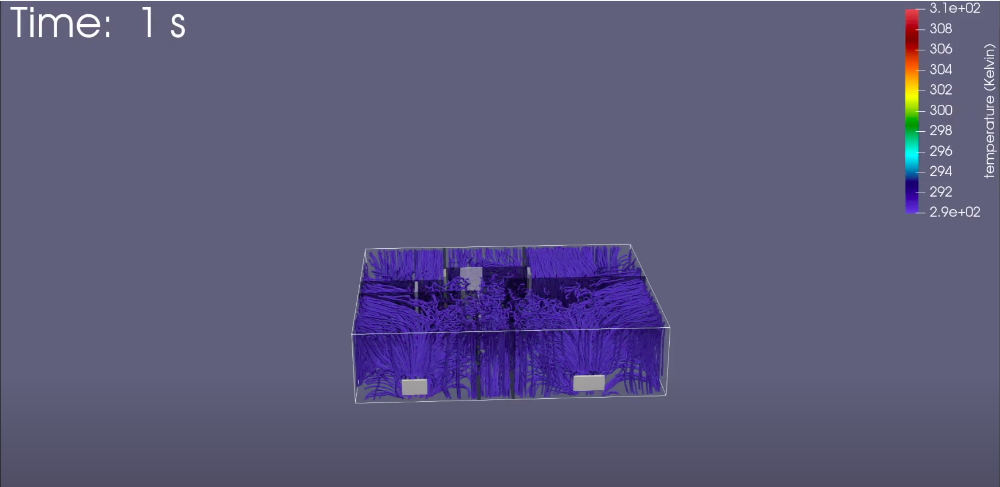
\includegraphics[width=\linewidth]{"images/cemosis_simulation_1.png"}
	\end{minipage} \hfill
	\begin{minipage}[t]{0.48\linewidth}
		\centering
		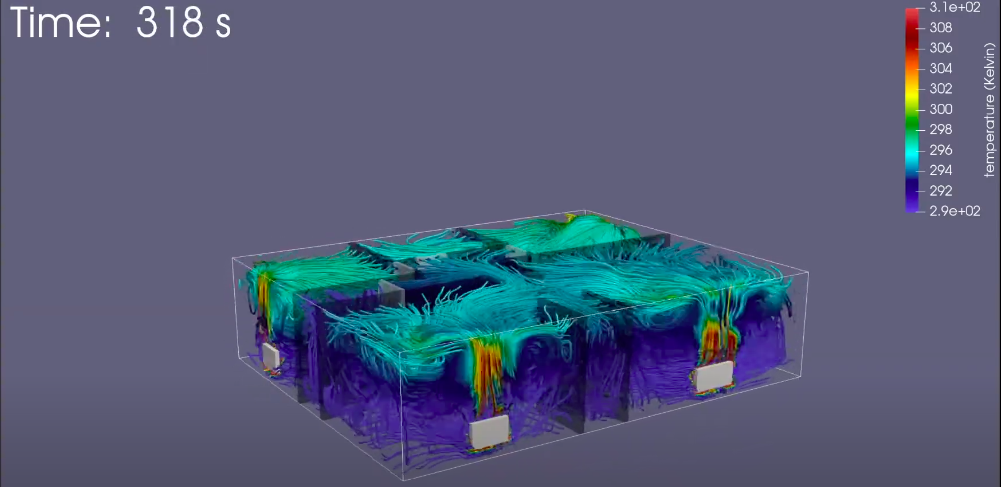
\includegraphics[width=\linewidth]{"images/cemosis_simulation_2.png"}
	\end{minipage}
	\captionof{figure}{Example of a building simulation with Feel++}
    \end{figure}
	
	\subsection{Goals of the Intership}
	\noindent The main objective of the intership is to implement the Parareal method and data assimilation for PDEs with Feel++. 
	\newline
	
	\noindent \textbf{Objectives for the common part}:
    	\begin{enumerate}
        \item To read the following article about the Heat equation (Chapter 11) : \cite{quarteroni_numerical}
			\item To set up a project on Github :
			\begin{itemize}
				\item Organisation of the repository (Python library, cmake in C++ ...)
				\item Create issues to see the progress of the project
				\item Set up the CI : build, test, documentation 
			    \end{itemize}\; \\
		Github repository : \url{https://github.com/master-csmi/2022-m1-lorenz}
	\end{enumerate}
	
	\noindent \textbf{Objectives for parareal method:}
	\begin{enumerate}
		\item Implement the parareal method in C++ and :
		\begin{itemize}
			\item Test the method (with oscillator)
			\item Check convergence and stability results
			\item Check speed-up and efficiency 
		\end{itemize}
		\item Implement the resolution of the heat equation in C++ with Feel++ \\
		$\Rightarrow \quad $ Implement the resolution of the Laplace equation in C++ with Feel++
		\item Use the previous implementation of the heat equation with the parareal method
		\item Check the convergences/accuracies of the method
	\end{enumerate}
	\newpage
	\noindent \textbf{Objectives for the Data assimilation:}
	\begin{enumerate}
        \item Write a class for the EnKF in C++, inspired by the EnKF written in Python (FilterPy); Test the algorithm.
        \item To read the following article :
        \begin{itemize}
            \item Fundamentals Of Building Performance Simulation By Beausoleil-Morrison
        \end{itemize}
        
    \item Understand the heat equation and what are the phenomena involved in the modification of the temperature of a building (conduction, convection, radiation).
    \item Write the mathematical problem to be solved if we want to simulate an office then realize the simulation using Feel++ toolboxes.
    \item Introduce data assimilation using the sensor and correct the simulation.
    \end{enumerate}

	\newpage

	\section{Differential Equations}
	\noindent In Mathematics, ordinary differential equations (ODE) are equations that involve derivatives of one-variable functions, and partial differential equations (PDE) are equations that imposes relations between the various partial derivatives of a multivariable function.
	The difference between ODEs and PDEs is that for ODEs the unknown functions depend only on one variable, whereas for PDEs the unknown functions may depend on several independent variables.
	\noindent Differential equations are an important object of study in both pure and applied mathematics. They are used to build mathematical models of physical and biological evolution processes, for example for the study of radioactivity, celestial mechanics, weather or population dynamics... 
	\noindent During the project we had already used the Lorenz system and the harmonic oscillator, for the internship we also used these two differential equations but we worked with two other equations: the heat equation and the Laplacian.
	
	\subsection{ODE: Harmonic oscillator}
	\label{oscillator_ode}
	\noindent A harmonic oscillator is an ideal oscillator whose evolution over time is described by a sinusoidal function, whose frequency depends only on the characteristics of the system and whose amplitude is constant.This mathematical model describes the evolution of any physical system in the vicinity of a stable equilibrium position, which makes it a transversal tool used in many fields: mechanics, electricity and electronics, optics.
	\begin{figure}[H]       
	\begin{minipage}[t]{0.46\linewidth}
		\centering
		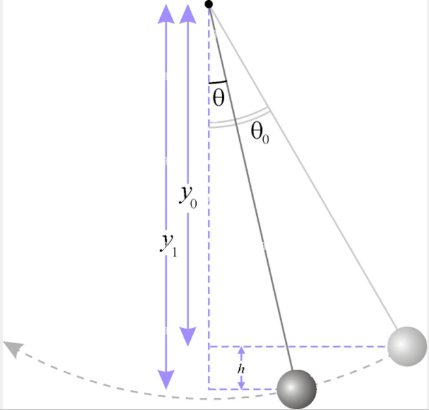
\includegraphics[width=\linewidth]{"images/Diff_equation/Harmonic_oss_1.png"}
		\captionof{figure}{Simple pendulum}
	\end{minipage} \hfill
	\begin{minipage}[t]{0.48\linewidth}
		\centering
		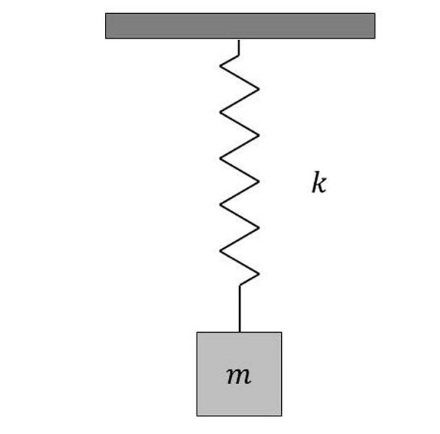
\includegraphics[width=\linewidth]{"images/Diff_equation/Harmonic_oss_2.png"}
		\captionof{figure}{Spring/mass system}
	\end{minipage}
    \end{figure}
	
	\newpage
	
	\noindent Let's consider a mass-spring system of the following form :

    \begin{equation}
    	\frac{d^2 x}{d t^2}+\omega_0^2 x = 0 \quad \iff \quad \frac{d^2 x}{d t^2}=-\omega_0^2 x \quad \text{with} \quad \omega_0=\sqrt{\frac{k}{m}}.
    	\label{osc}
    \end{equation}
    
    \noindent $k$ and $m$ are the spring stiffness and the suspended mass respectively. We are interested in this equation because its exact solution is known and is of the form :
    $$x(t) = x_0 \cos(\omega_{0}t+\phi_0).$$
    
    \noindent First of all, the numerical methods such as Runge Kutta order 4  allow us to solve first order differential equations. But the harmonic oscillator equation (\ref{osc}) is a second order equation. We will therefore start by making a simple change of variable which will allow us to replace this second order differential equation by a system of two first order equations. We pose :
     
    $$\qquad \frac{d x}{d t}=v \quad \Rightarrow \quad \frac{d^2 x}{d t^2}=\frac{d v}{d t}.$$
    
    \noindent As a result the equation becomes :
    
    $$\left\{\;\begin{aligned}
    	\frac{d x}{d t}&=v \\
    	\frac{d v}{d t}&=-\omega_0^2 x
    \end{aligned}\right.
    $$
    
    \noindent Let's take an example to understand how we can determine the exact solution from the initial conditions that we will take. For example if we take $\omega_0=5$ and $(x(0),v(0))=(0,1)$, we have :
    
    $$\left\{\;\begin{aligned}
    	x(0)&=0 \\
    	v(0)&=1
    \end{aligned}\right. \quad \Rightarrow 
    \left\{\;\begin{aligned}
    	x_0 \cos(\phi_0)&=0 \\
    	-x_0 \omega_{0} \sin(\phi_0)&=1
    \end{aligned}\right.  \quad \Rightarrow  
    \left\{\;\begin{aligned}
    	x_0&=\frac{-1}{5} \\
    	\phi_0&=\frac{\pi}{2}
    \end{aligned}\right.
    $$
    
    \noindent And thus the solutions of the equation are of the form :
    
    $$x(t) = \frac{-1}{5}\cos(5t+\frac{\pi}{2}).$$
    \subsection{ODE: Lorenz system}
	\label{lorenz_ode}
	\noindent The Lorenz system is a simplified three-variable model to investigate atmospheric convection. This model has had important repercussions in showing the possible limits on the ability to predict long-term climate and weather evolution. One of the important characteristics of the Lorenz system is 
	that it is a chaotic system, which means that this type of system is roughly defined by sensitivity to initial conditions: infinitesimal differences in initial conditions of the system result in large differences in behavior.
	\begin{figure}[H]   
		\centering
		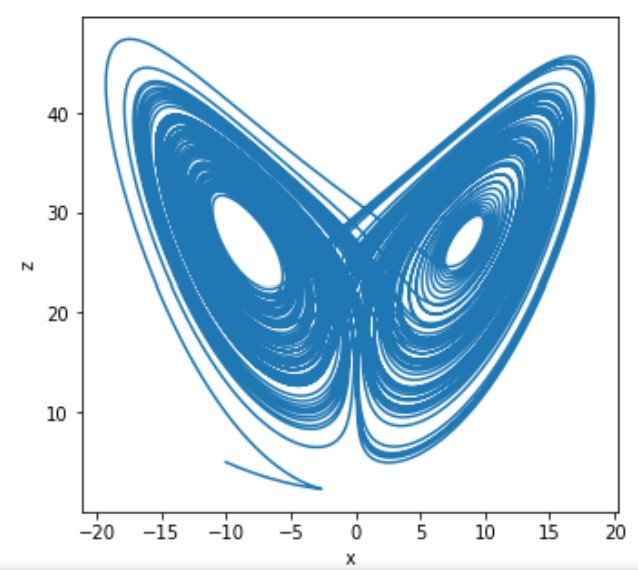
\includegraphics[width=0.5\textwidth]{"images/butterfly.jpg"}
		\caption{butterfly wing pattern}
		\label{but_wing}
	\end{figure}	
	
	\noindent The Lorenz system defines a 3 dimensional trajectory by differential equations with 3 parameters.
	$$
	\begin{cases}
		
		x'&=\sigma(y-x) \\
		y'&=x(r-z)-y \\
		z'&=xy-bz
		
	\end{cases}
	$$
	
	\noindent Here, $x$ is proportional to the rate of convection, $y$ is related to the horizontal temperature variation, and $z$ is the vertical temperature variation.
	We have also three parameters all strictly positive:
	\begin{enumerate}[label=\textbullet]
		\item $\sigma > 0$  relates to the Prandtl number. This number is a dimensionless quantity that puts the viscosity of a fluid in correlation with the thermal conductivity;
		\item $r > 0$  relates to the Rayleigh number, it is a control parameter, representing the temperature difference between the top and bottom of the tank;
		\item $b > 0$ relates to the physical dimensions of the layer of fluid uniformly heated from below and cooled from above.
	\end{enumerate}
	
	\noindent We can see that this system is non-linear, because in the second differential equation ( $\frac{dy}{dt}$) we can see the term $xz$ and in the third differential equation ($\frac{dz}{dt}$) we have $xy$. The three differential equations form a coupled system. 
	
	\noindent Let us now determine the fixed points of the Lorenz system. These are the points such that $X'=0$. 
	
	$$
	X'=(x',y',z')=0
	\quad \Rightarrow \quad 
	\left\{\begin{aligned}
		x'=&\sigma(y-x) &&=0 \\
		y'=&x(r-z)-y  &&=0\\
		z'=&xy-bz &&=0
	\end{aligned}\right. 
	\quad \Rightarrow \quad 
	\left\{\begin{aligned}
		&x=y \\
		&(r-1-z)x=0\\
		&x^2=bz
	\end{aligned}\right.
	$$
	
	\begin{enumerate}[label=\textbullet]
		\item If $x=0$ : \quad  $y=0$ and $z=0$.
		\item If $x\ne 0$ and $r>1$ : \quad $\left\{\begin{aligned}
			&z=r-1\\
			&x=y=\pm\sqrt{b(r-1)}
		\end{aligned}\right.
		$
	\end{enumerate}
	
	\noindent We deduce that the fixed points of the Lorenz system are: $(0,0,0)$ for all values of the parameters. And for $r>1$, there is also a pair of fixed points $(\sqrt{b(r-1)},\sqrt{b(r-1)},r-1)$ and $(-\sqrt{b(r-1)},-\sqrt{b(r-1)},r-1)$.
	
	\subsection{PDE: Laplacian equation}
	\label{laplacian_pde}
    \noindent The Laplace equation is a second-order partial differential equation . This equation is a basic PDE that arises in the heat and diffusion equations. It is a useful method for determining electric potentials in space or the free region.
    It is often written as :
    $$\Delta f=0 \qquad \text{or} \qquad \nabla^2 f=0$$
    \noindent with $\Delta$ the Laplace operator. We can define the Laplace operator as follows: $\Delta=\nabla \cdot \nabla$ where $\nabla \cdot$ divergence operator and $\nabla$  is the gradient operator.
    
    \noindent We can write the problem this way:
    
	$$\left\{\begin{aligned}
		-\Delta u &= f \quad&&\Omega \\
		u&=g \quad&&\Gamma_D \\
		\frac{\partial u}{\partial n} &=h \quad &&\Gamma_N \\
		\frac{\partial u}{\partial n}+u &=l \quad &&\Gamma_R \\
	\end{aligned}\right.$$
	\noindent Where $\Omega$ corresponds to our domain, $\Gamma_D$  corresponds to the Dirichlet boundary condition, $\Gamma_N$ to the Neumann boundary condition and $\Gamma_R$ to the Robin boundary condition.
	\subsection{PDE: Heat equation}
	\label{heat_pde}
	\noindent Heat transfer is the process of energy transfer resulting from a temperature difference. 
	\newline
    \noindent Thermal analysis is undertaken to predict temperatures and heat transfer in and around bodies. This information can then be used to model temperature-dependent phenomena, such as heat-induced stresses or the effect on fluid flow in the case of a solidifying metal.  Heat flow has been classified into three different modes: conduction, convection and radiation.
    \begin{figure}[H]       
	\begin{minipage}[t]{0.45\linewidth}
		\centering
		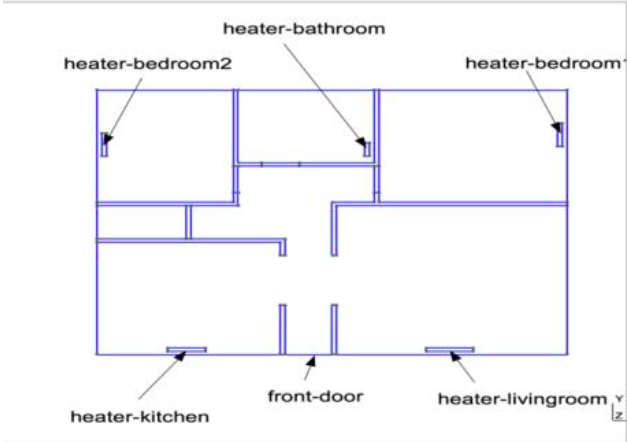
\includegraphics[width=\linewidth]{"images/Diff_equation/heat_1.png"}
	\end{minipage} \hfill
	\begin{minipage}[t]{0.50\linewidth}
		\centering
		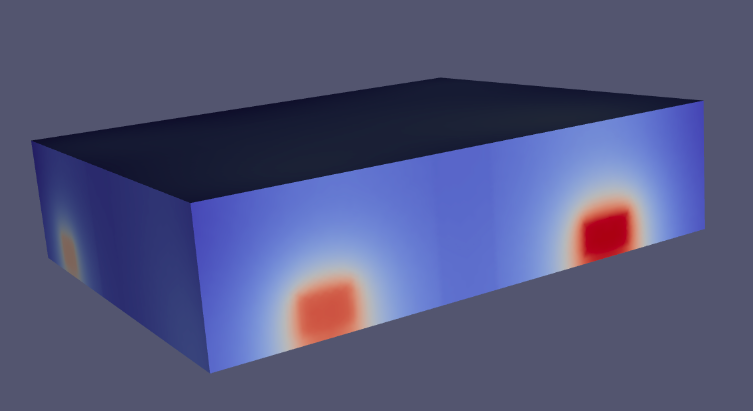
\includegraphics[width=\linewidth]{"images/Diff_equation/heat_2.png"}
	\end{minipage}
	\captionof{figure}{Simulation of the temperature of a building using the heat equation with Feel++}
    \end{figure}


	\noindent The heat equation with convective effects can be written as:
    $$\rho C_p((\frac{\partial T}{\partial t})+u . \nabla T)-\nabla .(k \nabla T)=Q$$
    and it must be completed  with boundary conditions and initial conditions.
    \newline
	\renewcommand{\arraystretch}{2}
    \begin{tabular}{|R{3cm}|C{3cm}|L{3cm}|L{3cm}|}
    \hline
    Notation & Quantity &Unit & Value   \\
    \hline
    $\rho$ & density & $Kg.m^
    {-3}$ & 1.125  \\[4cm]
    \hline
    $C_p$ & Specific heat & $J/KgC=J/KgK$ & 1004 \\[4cm]
    \hline
    $k$ & Conductivity & $W/mC=W/mK$ & 0.025 \\[4cm]
    \hline
    $u$ & Fluid velocity & $m.s^{-1}$  & unknown \\[4cm]
    \hline
    $T$ & Temperature & $K$ or $C$  & unknown \\[4cm]
    \hline
    $t$ & Time & s. &   \\[4cm]
    \hline
\end{tabular}

	\newpage

    \subsection{Runge-Kutta}
    \label{rk4}
    \noindent During our project and internship we used the Runge-Kutta method of order 4 to solve ordinary differential equations. Runge-Kutta techniques are one-step numerical schemes for solving ordinary differential equations. They are among the most popular methods because of their ease of implementation and accuracy.
    
    \noindent We consider $f : [0; T] \times \mathbb{R}^n \rightarrow \mathbb{R}^n$ a continuous function. For $X_0\in \mathbb{R}^n$, the problem is to find  $X\in C^1([0,T],\mathbb{R}^n)$ solution for the differential equation:
	
	$$\left\{\begin{aligned}
		X'&=f(t,X), \\
		X(0)&=X_0.
	\end{aligned}\right.$$
	
	
	 \noindent After discretizing the problem in time, we can use the Runge Kutta method of order 4 to solve the ODE:
		
		$$X_{n+1}=X_n+\frac{\Delta t}{6}\left(K_1+2K_2+2K_3+K_4\right) ,$$
		
		\noindent where 
		
		$$\left\{\begin{aligned}
			K_1&=f(t_n,X_n) , \\
			K_2&=f\left(t_n+\frac{\Delta t}{2},X_n+\frac{1}{2} K_1\Delta t\right) , \\
			K_3&=f\left(t_n+\frac{\Delta t}{2},X_n+\frac{1}{2} K_2\Delta t\right) , \\
			K_4&=f\left(t_n+\Delta t,X_n+K_3\Delta t\right) .
		\end{aligned}\right.$$
	
    

	%\noindent For the next part of the project, we choose to work with the Runge kutta method.
	
	\newpage
	
	\begin{frame}{What is the parareal method ?}
	
	\begin{enumerate}[\textbullet]
		\item parallel-in-time integration method, introduced in 2001 by Lions, Maday and Turinici
		\item computes the numerical solution for multiple time steps in parallel
		\item categorized as a parallel-across-the-steps method 
	\end{enumerate}

\end{frame}

\begin{frame}{Objectives for parareal method}
	
	\begin{enumerate}[\textbullet]
		\item Implement the parareal method in C++ and :
		\begin{itemize}
			\item Test the method (with oscillator)
			\item Check convergence and stability results
			\item Check speed-up and efficiency 
		\end{itemize}
		\item Implement the resolution of the heat equation in C++ with Feel++ \\
		$\Rightarrow \quad $ Implement the resolution of the Laplace equation in C++ with Feel++ \\
		\item Use the previous implementation of the heat equation with the parareal method
		\item Check the convergences/accuracies of the method
	\end{enumerate}
	
\end{frame}


\subsection{Theory}

\begin{frame}{Generalities of the parareal method}
	Time decomposition :
	\begin{enumerate}[\textbullet]
		\item $[t_0,T]=[t_0,t_1]\cup\dots\cup[t_{P-1},t_P]$ with $t_P=T$ and $P=$ number of processes
	\end{enumerate}

	\; \\

	\begin{minipage}{\linewidth}
		Notations :
		\begin{enumerate}[\textbullet]
			\item $F$ : high accuracy integrator, \quad $\Delta t_F$ : time step \\
			$G$ : low accuracy integrator, \quad $\Delta t_G$ : coarse time step
			\item $U_j^k, j\in\{0,\dots,P\}$ : initial point at time $t_j$ and at iteration $k$.
		\end{enumerate}
	\end{minipage} \\
	\begin{enumerate}[\textbullet]
		\item $F(U_{j-1}^k), j\in\{1,\dots,P\}$ : value of the fine integrator at $t_j$ starting by $U_{j-1}^k$ (resp. $G(U_{j-1}^k)$)
	\end{enumerate}
	\begin{minipage}{\linewidth}
		\centering
		\qquad \qquad \qquad \qquad \qquad \qquad \qquad 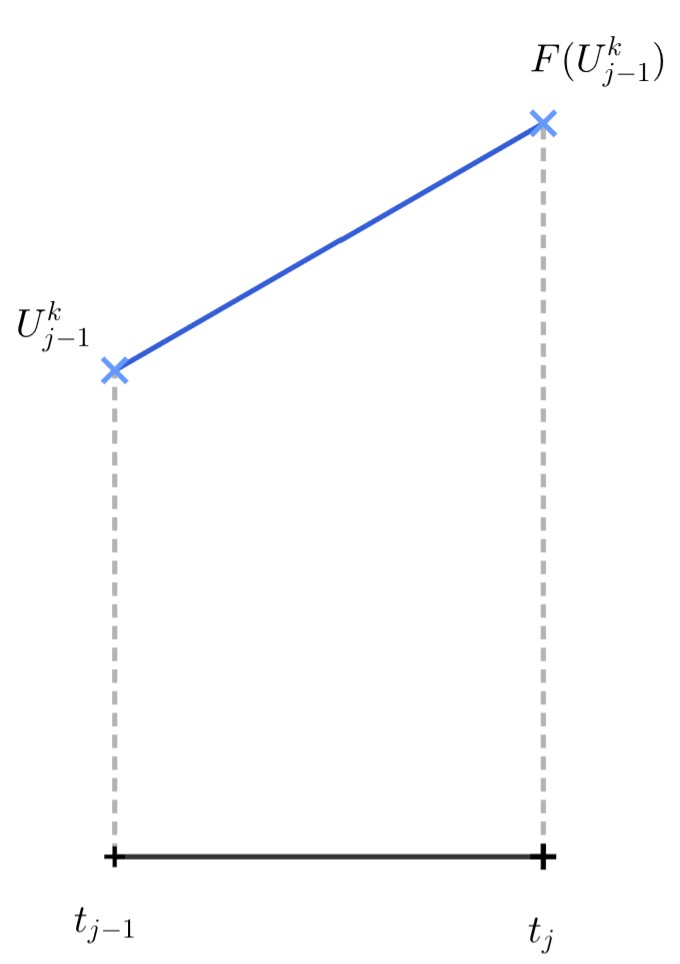
\includegraphics[width=0.35\linewidth]{images/parareal/explane_F.jpg}
	\end{minipage}
	
\end{frame}

\begin{frame}[allowframebreaks]{Explanation of the parareal method}
	\begin{figure}
		\centering
		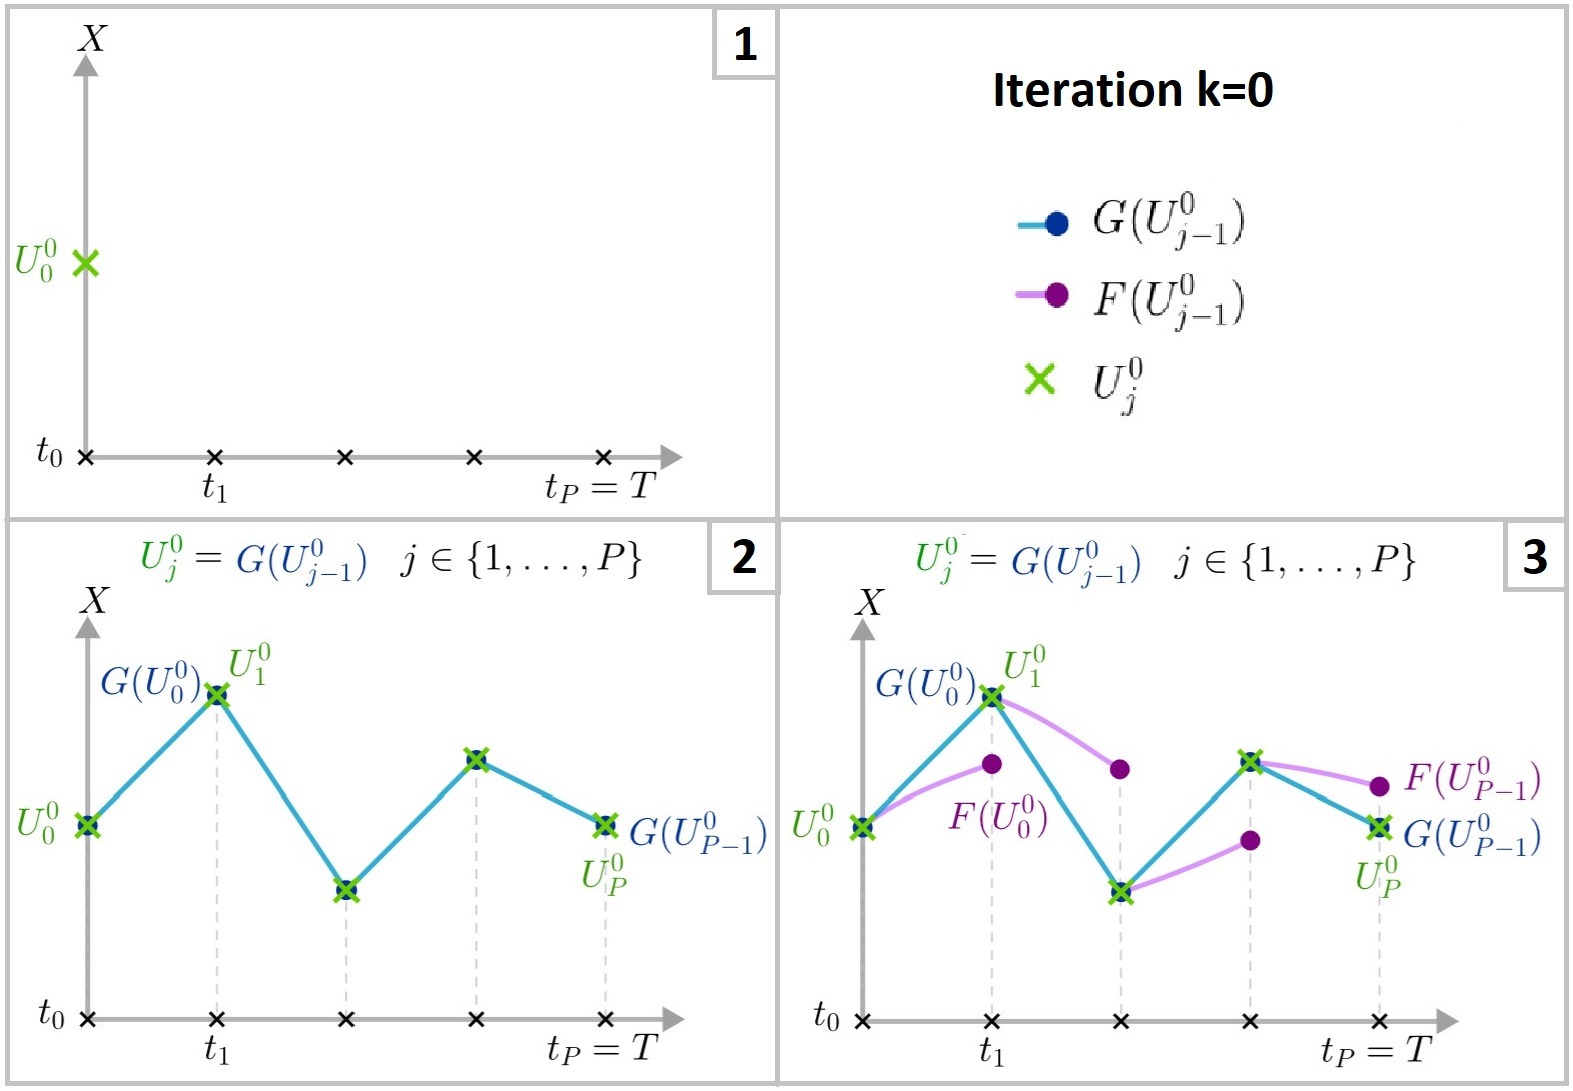
\includegraphics[width=0.6\linewidth]{images/parareal/parareal_k0.jpg}
		\caption{Explanation of the parareal method at iteration $k=0$ (step 1 to 3)}
	\end{figure}
	\begin{figure}
		\centering
		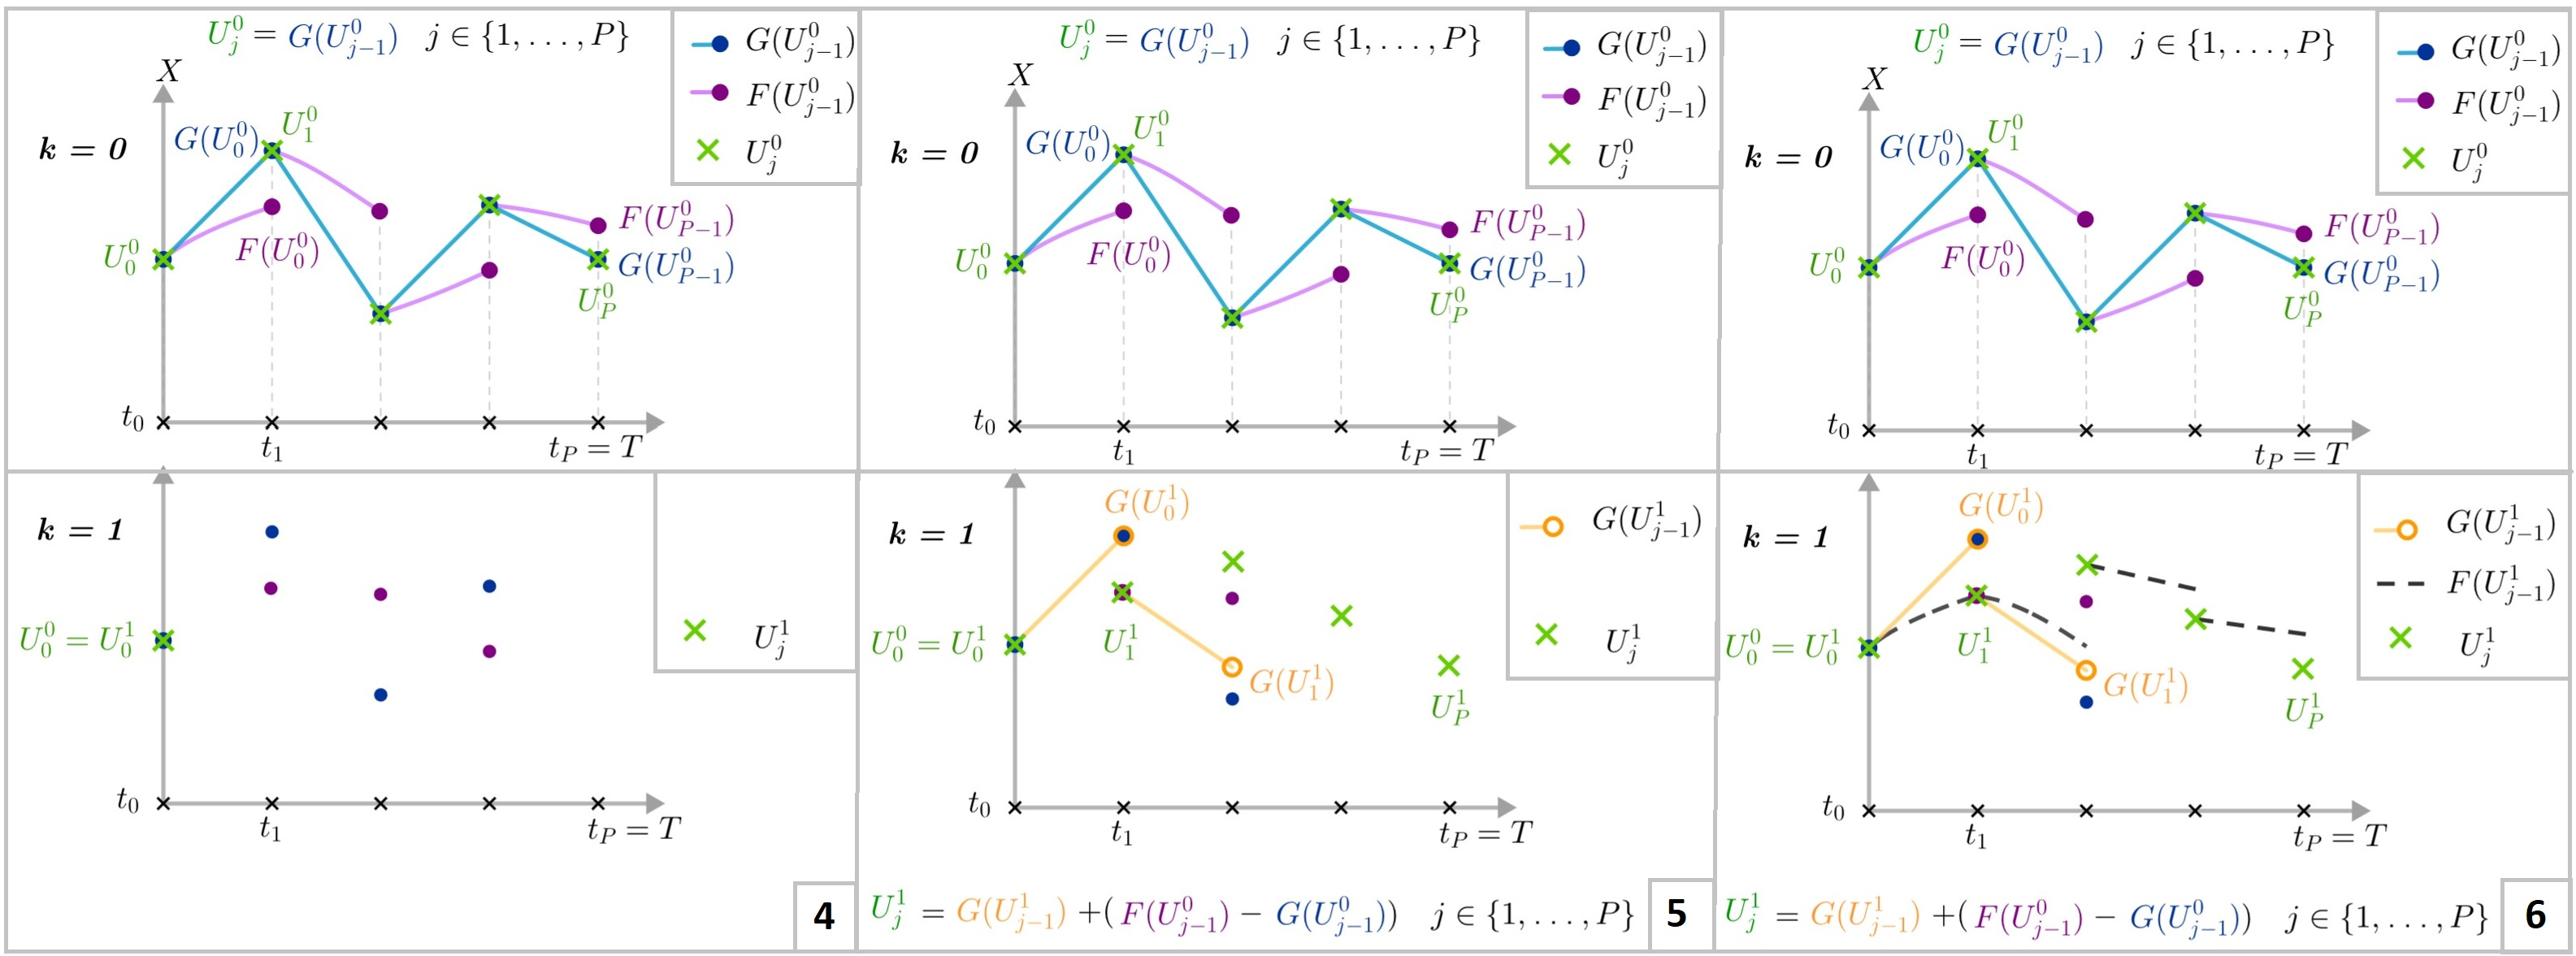
\includegraphics[width=0.9\linewidth]{images/parareal/parareal_k1.jpg}
		\caption{Explanation of the parareal method at iteration $k=1$ (step 4 to 6)}
	\end{figure}
	\small
	We have at iteration $k$ : \qquad	$U_j^k=G(U_{j-1}^k)+(F(U_{j-1}^{k-1})-G(U_{j-1}^{k-1}))$
\end{frame}

\begin{frame}{Example with the Lorenz system}
	\centering
	$\sigma=10, \quad b=\frac{8}{3}, \quad r=28, \quad X_0=(5,5,5), \quad t_0=0, \quad T=20$
	$P=4,\quad \Delta t_G=0.1, \quad \Delta t_F=0.01$
	\begin{figure}
		\centering
		\begin{minipage}{0.48\linewidth}
			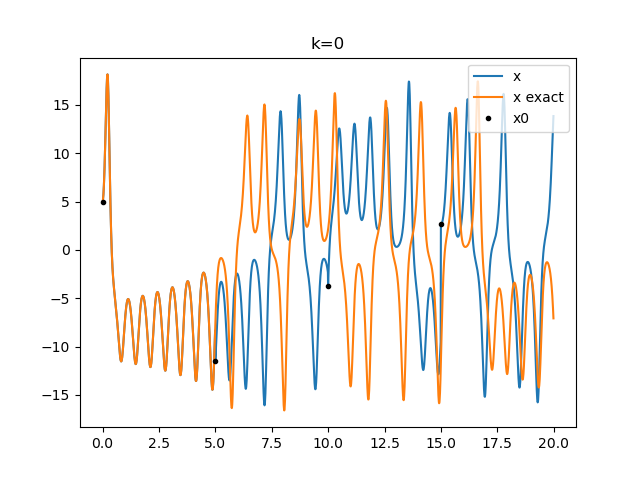
\includegraphics[width=\linewidth]{"images/parareal/lorenz_sol_0.png"}
		\end{minipage}
		\begin{minipage}{0.48\linewidth}
			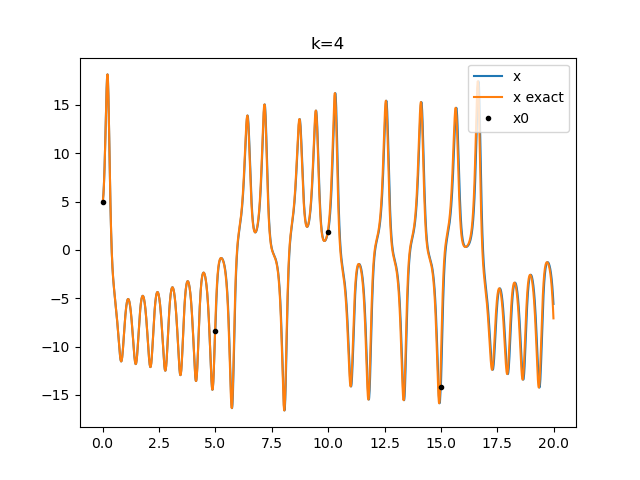
\includegraphics[width=\linewidth]{"images/parareal/lorenz_sol_4.png"}
		\end{minipage}
		\caption{Solution of the Lorenz system at the first and the last iteration (with C++)}
	\end{figure}
\end{frame}

\begin{frame}{Order of the parareal method}
	The parareal method is of order k if there is a constant $c_k$ such that :
	\begin{equation*}
		\forall j\in\{0,\dots,P-1\} \qquad \mathcal{E}(j,k)\le c_k(\Delta t_G)^k
	\end{equation*}
	with
	$$\mathcal{E}(j,k)=|U_j^k-U_{ex}(t_j)|+\max_{t\in[t_j,t_{j+1}]}|U_k(t)-U_{ex}(t)|$$
	\begin{figure}
		\centering
		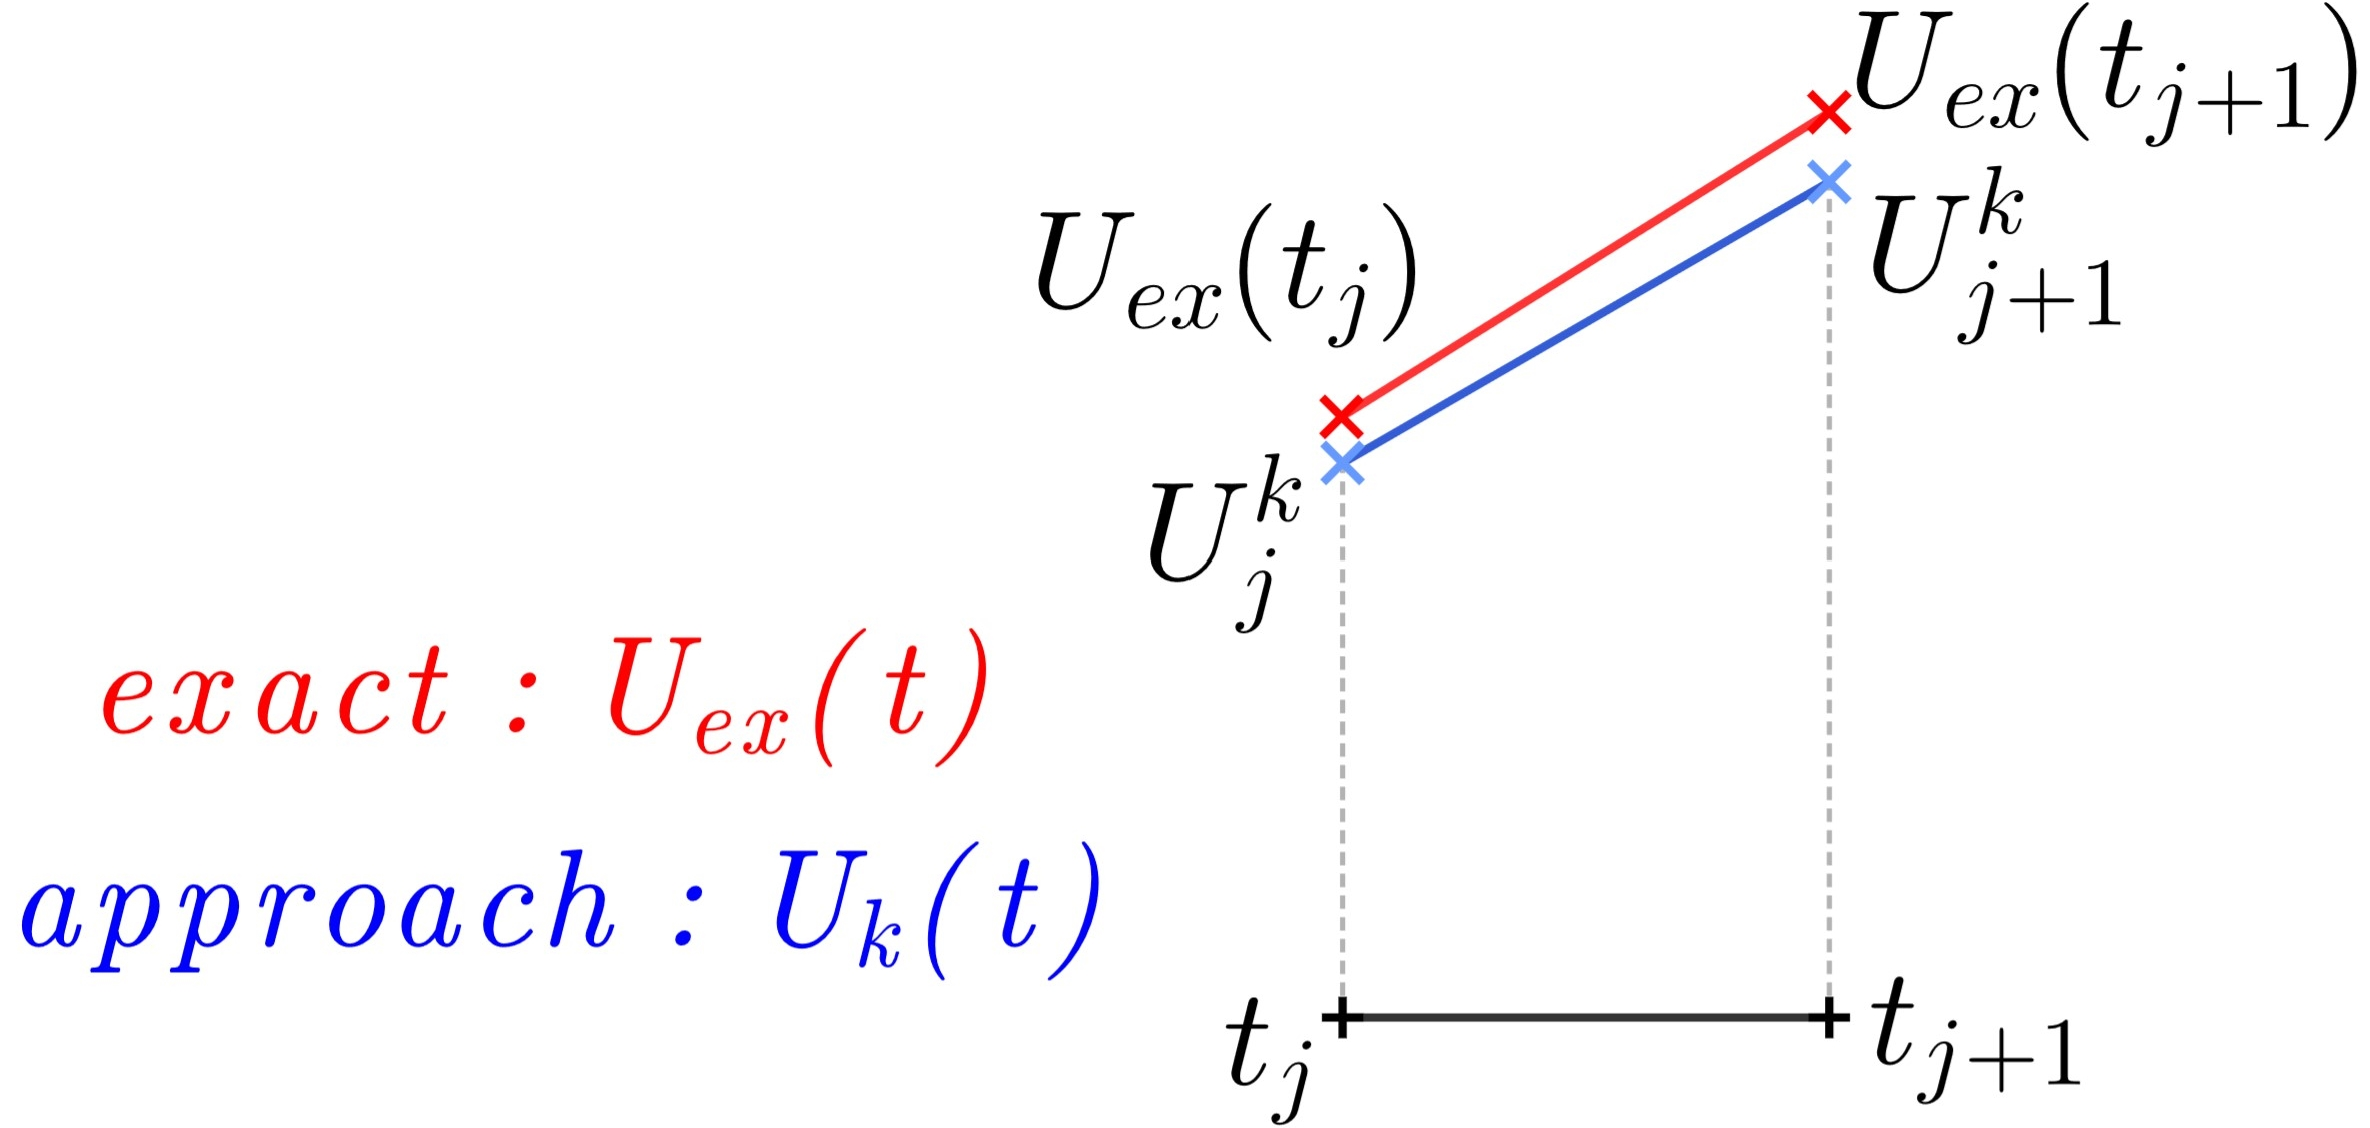
\includegraphics[width=0.62\linewidth]{images/parareal/explane_order.jpg}
		\caption{Explanation of the order property}
	\end{figure}
\end{frame}


\begin{frame}{Harmonic oscillator}
	
	$$P=3, \quad x(0)=0,\quad v(0)=1, \quad\omega_0=5, \quad x_0=\frac{-1}{5}, \quad \phi_0=\frac{\pi}{2}$$
	
	\begin{minipage}{0.45\linewidth}
		\begin{figure}
			\centering
			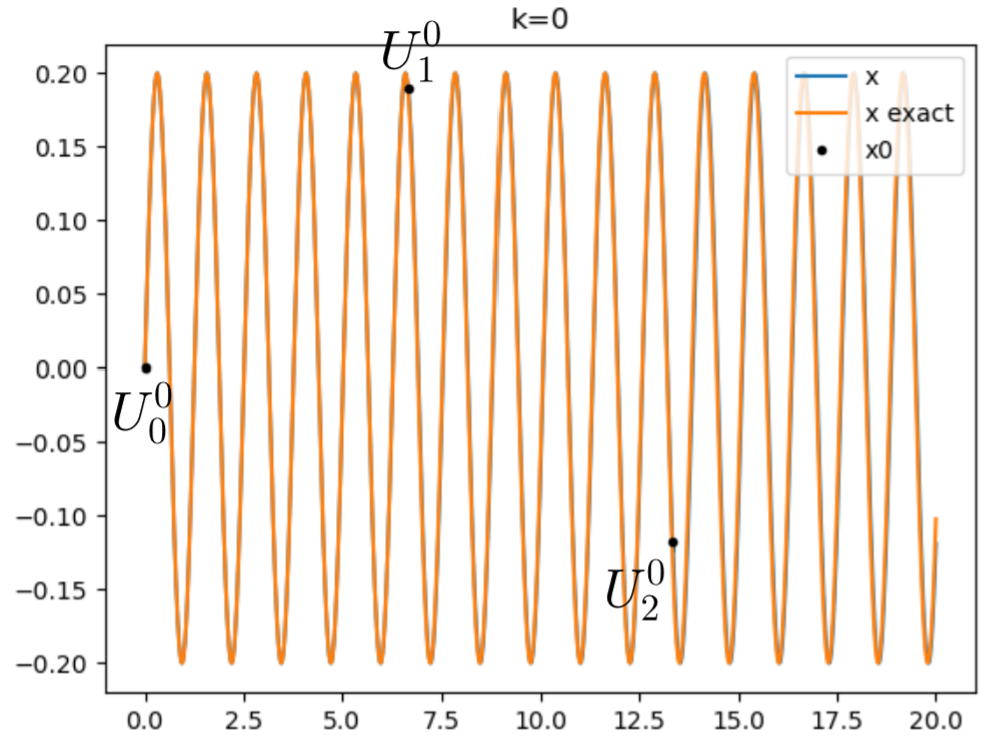
\includegraphics[width=\linewidth]{"images/parareal/osci_sol.png"}
			\caption{Parareal method applied to the harmonic oscillator (with C++)}
		\end{figure}
	\end{minipage} \; \qquad
	\begin{minipage}{0.45\linewidth}
		\begin{figure}
			\centering
			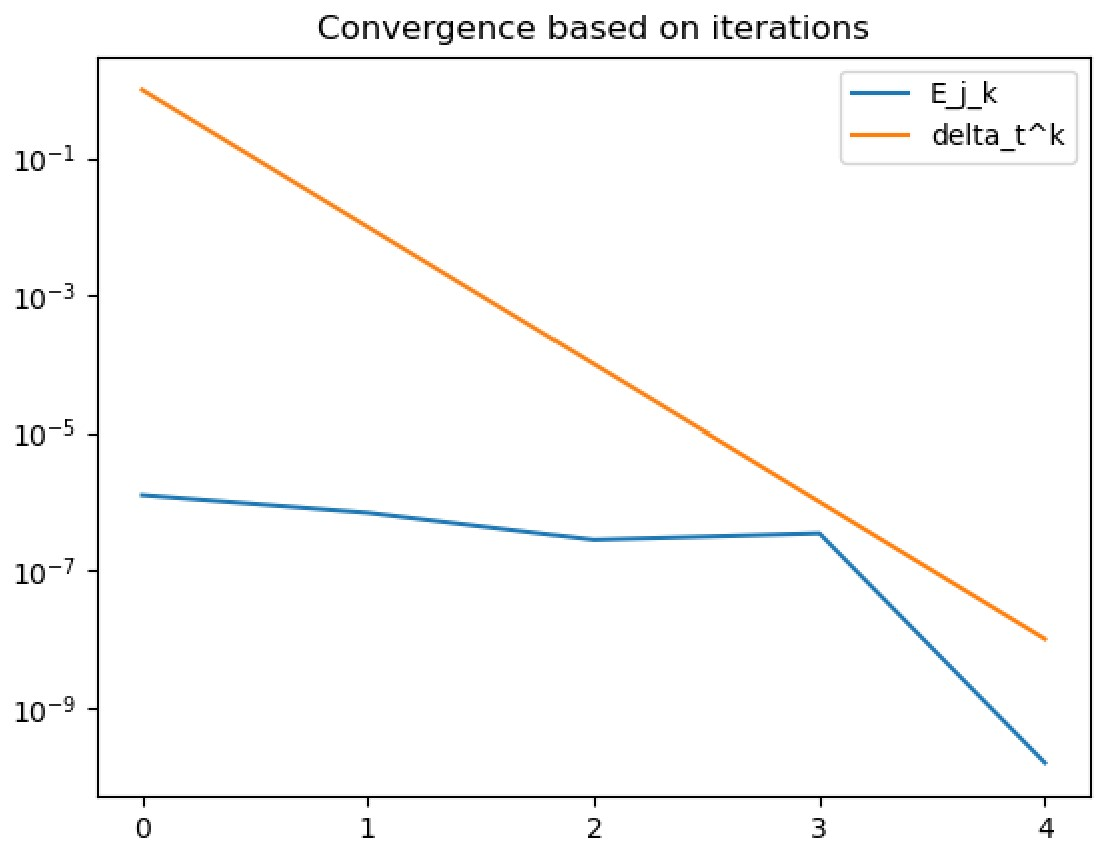
\includegraphics[width=\linewidth]{"images/parareal/osci_cvg_1.jpg"}
			\caption{Convergence property of parareal method with the harmonic oscillator (with Python)}
		\end{figure}
	\end{minipage}
	
\end{frame}

\begin{frame}{Speed-up ?}
	\begin{enumerate}[\textbullet]
		\item Why use this method ? \\
		Useful if the number of iteration is lower than $P$. \\
		
		\item We can see that the implementation of the method in C++ is considerably faster than in Python. \\
		
		\item Speed-up when we increase the number of processes $P$ ? \\
		With Python :
		\begin{table}[H]
			\centering
			\begin{tabular}{| c || c | c | c | c | c |}
				\hline
				\multirow{2}{1.5 cm}{$\Delta t$} & \multirow{2}{1.5 cm}{Seq (RK4)} & \multirow{2}{1.5 cm}{1 proc} & \multirow{2}{1.5 cm}{2 proc} & \multirow{2}{1.5 cm}{3 proc} &\multirow{2}{1.5 cm}{4 proc} \\
				& & & & & \\
				\hline 
				F : 0.00125 & \multirow{2}{1.5 cm}{1m19} & \multirow{2}{1.5 cm}{1m42} & \multirow{2}{1.5 cm}{39s} & \multirow{2}{1.5 cm}{32s} & \multirow{2}{1.5 cm}{29s} \\
				G : 0.0125 & & & & & \\	 
				\hline
			\end{tabular}
			\caption{Execution time for the Lorenz system with Python ($T=200$).}
			\label{time}
		\end{table}
	\end{enumerate}
\end{frame}






\subsection{Solving PDEs with Feel++}

\begin{frame}{Heat equation}
	
	\textbf{The problem :}
	$$\left\{\begin{aligned}
		\frac{\partial u}{\partial t}-\Delta u &= f \quad&&(t_0,T)\times\Omega \\
		u&=0 \quad&&(t_0,T)\times\partial\Omega\\
		u&=u_0 \quad &&\{0\}\times\Omega
	\end{aligned}\right.$$

	It describes the time evolution of the temperature $u$ of a medium contained in $\Omega$ under an external heat source $f$; $u_0$ is the initial temperature.
	
\end{frame}

\begin{frame}{Laplacian equation}
	
	\textbf{The problem :}
	$$\left\{\begin{aligned}
		-\Delta u &= f \quad&&\Omega \\
		u&=g \quad&&\Gamma_D \\
		\frac{\partial u}{\partial n} &=h \quad &&\Gamma_N \\
		\frac{\partial u}{\partial n}+u &=l \quad &&\Gamma_R \\
	\end{aligned}\right.$$
	
	\textbf{Weak formulation :} \\
	Find $\; u:\Omega \mapsto \mathbb{R} \;$ such that $\; u\in H_0^1(\Omega) \;$ and
	$$\int_\Omega \nabla u \cdot \nabla v + \int_{\Gamma_R}uv = \int_\Omega fv + \int_{\Gamma_N}hv+\int_{\Gamma_R}lv \quad \forall v\in H_0^1(\Omega)$$
	
\end{frame}

\begin{frame}[allowframebreaks]{Example with Laplacian}
	$$\left\{\begin{aligned}
		-\Delta u &= f \quad&&\Omega \\
		u&=g \quad&&\Gamma_D \\
	\end{aligned}\right. \quad \text{with} \quad
	u_{exact}=g=x^2+y^2, \quad f=-\Delta u_{exact}=-4$$
	\begin{minipage}{0.31\linewidth}
		\begin{figure}
			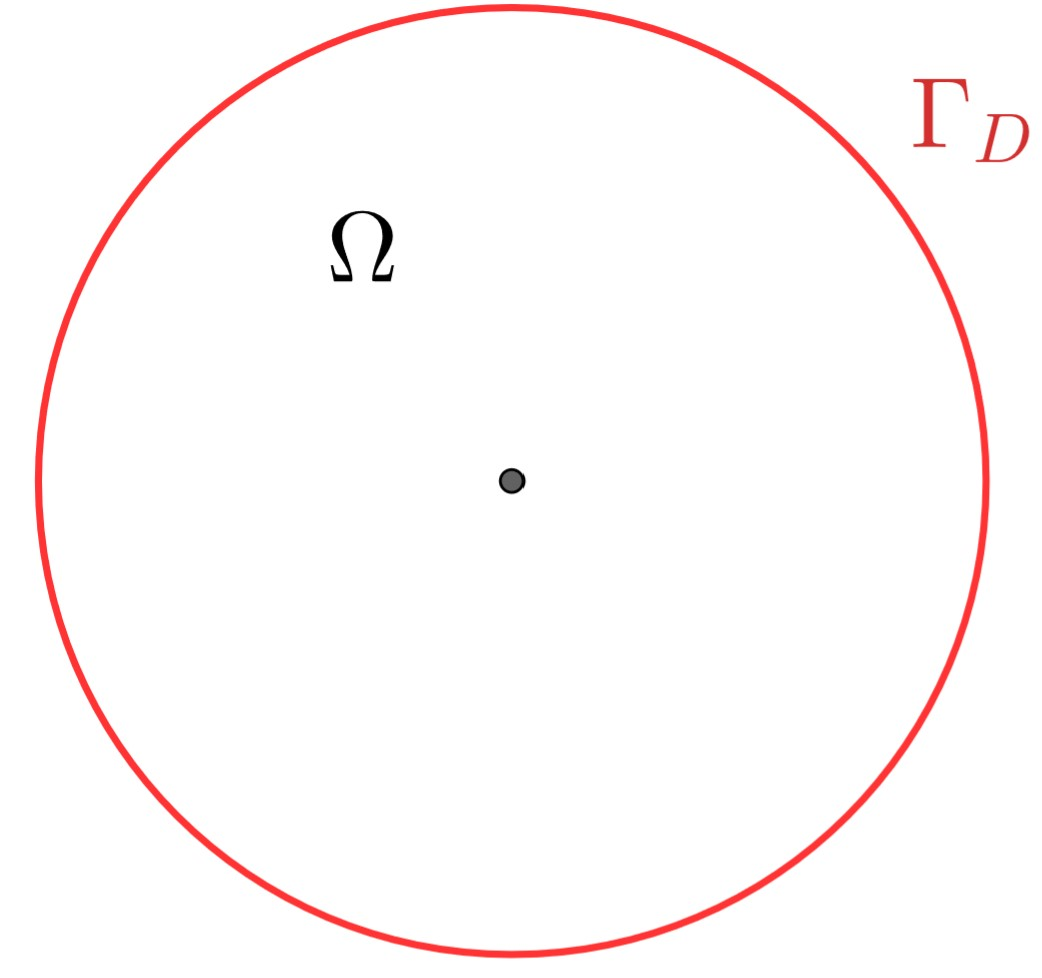
\includegraphics[width=\linewidth]{"images/parareal/circle.jpg"}
			\caption{Geometry considered}
		\end{figure}
	\end{minipage} \quad
	\begin{minipage}{0.31\linewidth}
		\begin{figure}
			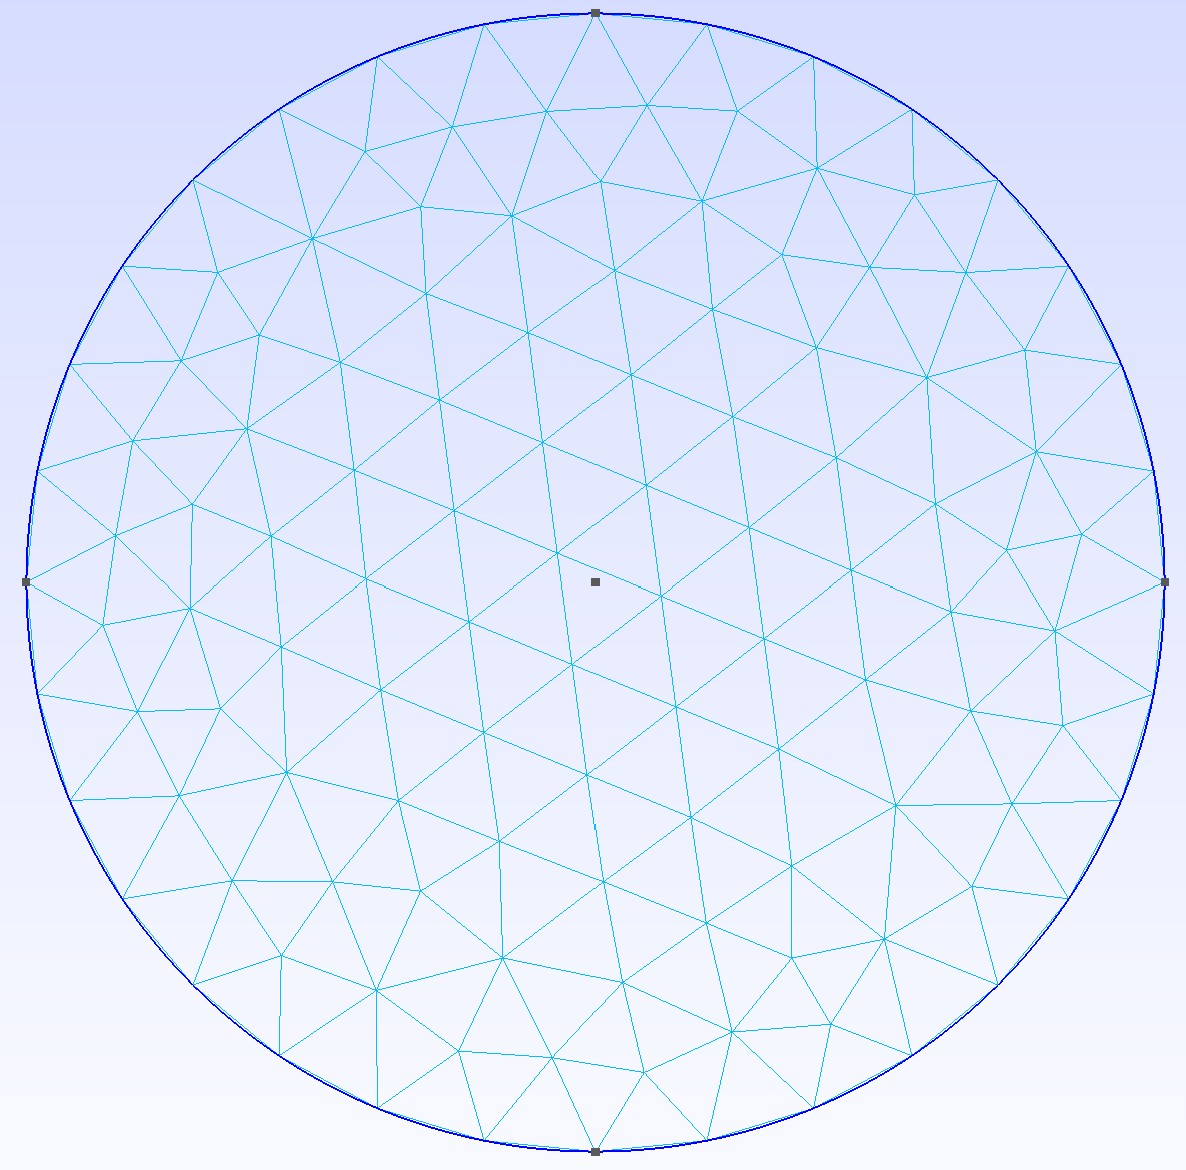
\includegraphics[width=\linewidth]{"images/parareal/circle_mesh.jpg"}
			\caption{Mesh of the geometry (with Dirichlet Boundary condition)}
		\end{figure}
	\end{minipage} \quad
	\begin{minipage}{0.31\linewidth}
		\begin{figure}
			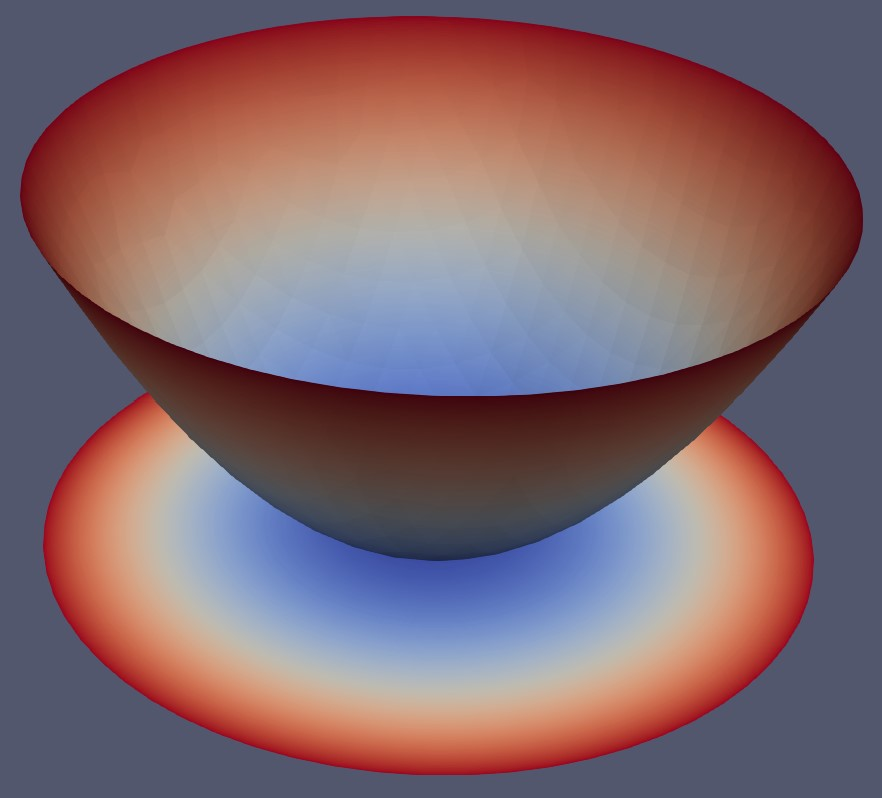
\includegraphics[width=\linewidth]{"images/parareal/circle_result.jpg"}
			\caption{Result (with Paraview)}
		\end{figure}	
	\end{minipage}

	\newpage
	\centering
	$||u-u_h||_{L^2}\sim h^2 \qquad \qquad ||u-u_h||_{H^1}\sim h^1 $
	\begin{figure}
		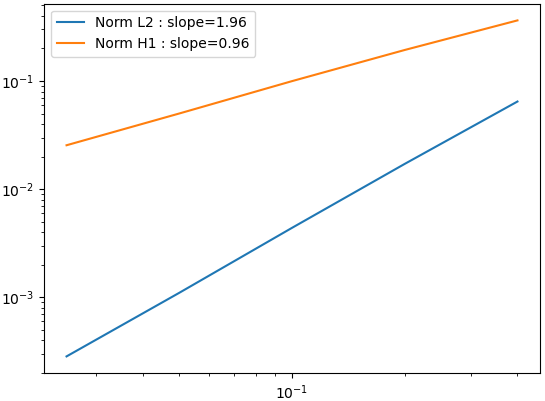
\includegraphics[width=0.52\linewidth]{"images/parareal/cvg_laplacian.png"}
		\caption{Convergence order for the Laplacian problem.}
	\end{figure}
\end{frame}

\begin{frame}{Back to the heat equation}
	\textbf{Weak formulation :} \\
	Find $\; u:(t_0,T)\times\Omega \mapsto \mathbb{R} \;$ such that $\; u(t,\cdot)\in H_0^1(\Omega) \;$ and
	$$\int_\Omega \frac{\partial u}{\partial t}(t,x)v(x)dx+\int_\Omega \nabla u(t,x)\cdot\nabla v(x)dx = \int_\Omega f(t,x)v(x)dx \quad \forall v\in H_0^1(\Omega)$$
	for almost every $t\in(0,T)$. \\
	
	
\end{frame}

\begin{frame}{Back to the heat equation}
	\textbf{Weak formulation :} \\
	Find $\; u:(t_0,T)\times\Omega \mapsto \mathbb{R} \;$ such that $\; u(t,\cdot)\in H_0^1(\Omega) \;$ and
	$$\boxed{\int_\Omega \frac{\partial u}{\partial t}(t,x)v(x)dx}+\int_\Omega \nabla u(t,x)\cdot\nabla v(x)dx = \int_\Omega f(t,x)v(x)dx \quad \forall v\in H_0^1(\Omega)$$
	for almost every $t\in(0,T)$. \\ \; \\
	
	need to manage the temporal discretizations \\
	$\Rightarrow$ use of the Feel++ bdf (Backward differencing formula) class :
	
	$$\int_\Omega \frac{\partial u}{\partial t}(t,x)v(x)dx \simeq \int_\Omega \frac{u^{n+1}(x)-u^n(x)}{\Delta t}v(x)dx$$
	
	(Backward Euler scheme)
\end{frame}

\begin{frame}{Parareal method with the Heat equation}
	\textbf{Goal :} To have a function that solves the heat equation between $t_i$ and $t_j$ with an initial condition (by using the previous resolution in C++ with Feel++) and apply the parareal method to it.
\end{frame}






	
	\newpage
	
	\section{Data assimilation}

\subsection{Intro}
\noindent Data assimilation is nowadays widely used to make predictions in complex systems, for example in weather forecasting or ocean prediction. Data assimilation is a method that combines observations with the output of a model to improve a prediction. 
The main idea is to combine information from our model and from observations, in order to have a more reliable analysis. Sometimes what you are trying to improve in your model may not be in the same space as what you observe this is something that you need to consider while doing your assimilation. It is also important to control our output, it is up to us to decide which input is responsible for the error in our output. This means that there will be uncertainties coming from the model or from the observations, these uncertainties coming from our input will also translate into uncertainties in our output.
At the end of this data assimilation we will have obtained an output which will be an estimate of the unknown quantity called the state variables.
The best estimate is searched for as a linear combination of the background estimate and the observations:

$$x^a=Lx^b+Ky^0$$


\noindent Data assimilation methods are often split into two families: variational methods and statistical methods.
The first method, called variational methods, consists in minimizing a cost function with the least squares approach. 
\subsection{statistical approach}
\subsubsection{Kalman filter}
The Kalman filter method consists in looking for $x^a$ an analysis, this analysis will be a linear combination of what we already know, our model and our observations.
To explain this method let's consider that we observe a single quantity, an estimation of a scalar quantity at a point in space.For example we are observing the temperature in the middle of the room, and the model also simulate the temperature in the middle of the room.  We will then have :
$$x^a=x^b+K(y-x^b)$$
with $x^a$ the analysis, $x^b$ the background or model, and $y$ the observation. 
We suppose that the true state $x^t$ exists so:
$$x^a-x^t+K(y-x^t-x^b+x^t)$$
let's define the errors:
$$\begin{aligned}
&\epsilon^a=x^a-x^t \\
&\epsilon^b=x^b-x^t \\
&\epsilon^y=y-x^t \\
\end{aligned}$$
So we will have:
$$\epsilon^a=\epsilon^b+K(\epsilon^y-\epsilon^b)$$
If we have many realisation of these error, then we will have:
$$<\epsilon^a>=<\epsilon^b>+K(<\epsilon^y>-<\epsilon^b>)$$
We want to have the analysis error variance as low as possible .So we want to minimize $<(\epsilon^a)^2>$ with respect to $K$ ,this will give us:
$$<(\epsilon^a)^2>=<(\epsilon^b)^2>+K^2<(\epsilon^y-\epsilon^b)^2>+2K<\epsilon^b(\epsilon^y-\epsilon^b)^2>$$
$$2k<(\epsilon^y)^2+(\epsilon^b)^2>-2<(\epsilon^b)^2>=0$$
\noindent We assume that the errors in the background and observation are uncorrelated.
$$K=\frac{<(\epsilon^b)^2>}{<(\epsilon^b)^2>+<(\epsilon^y)^2>} \Rightarrow K=\frac{(\sigma^b)^2}{(\sigma^b)^2+(\sigma^y)^2} $$
where $(\sigma^y)^2$ is the observation error variance and $(\sigma^b)^2$ is the background or model error variance.
\newline\noindent If we have $(\sigma^y)^2=0$, $K=1$ and $x^a=y$  this means that the observation are perfect.
\newline\noindent And if $(\sigma^b)^2=0$, $K=0$ and $x^a=x^b$ this is equivalent to ignoring the observations.
\vspace*{5mm}
\newline Now that we have explained the method for solving $x^a$ let's try to generalize our formula.

$$\left\{\begin{aligned}
		&x^a=(I-KH)x^b+Ky^0=x^b+K(y^0-H(x^b)) \\
        &K=BH^T(HBH^T+R)^{-1} \\
	\end{aligned}\right.$$
With $K$ the gain or weight matrix, $(y^0-H(x^b))$ the innovation and $H$ the linear model of the observations.
This formulation is called the Best Linear Unbiased Estimator(BLUE) or least squares analysis.
The principle of the Kalman filter is based on this formulation. Here is a small figure which illustrates the Kalman filter.
\vspace*{5mm}
\begin{center}
		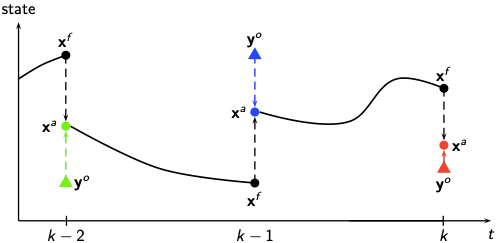
\includegraphics[width=0.8\textwidth]{"images/schema_kalman_filter.png"}
	\end{center}
The general idea consists in estimating the state at time $k$ from an estimate at time $k-1$ and measurements at time $k$.
We do the estimation in two steps:
\begin{enumerate}[label=\textbullet]
		\item Prediction of the state from the evolution model
		\item Correction of the prediction from the measurements
	\end{enumerate}

\subsubsection{Kalman filter algorithm}
For the notations we will use:

\noindent Vector:
 \begin{enumerate}[label=\textbullet]
		\item $k$ time index
		\item $x_{k}^{f}$ forecast state (background), forecast error covariance matrix $P_{k}^{f}$
		\item $x_{k}^{a}$ analyzed state (result of the assimilation process), analysis error covariance matrix $P_{k}^{a}$
	\end{enumerate}
\noindent Operators:
    \begin{enumerate}[label=\textbullet]
		\item model operator $x_{k+1}^{t} = M_{k,k+1}(x_{k}^{t})+ \eta
		_{k,k+1}$, model error $\eta
		_{k,k+1}$, covariance matrix $Q_k$
		\item observation operator $y_k^o = H_k (x^t ) + \epsilon_k^0$ , observation error $\epsilon^0$, covariance matrix $R_k$
	\end{enumerate}
\noindent The hypotheses necessary for the application of the Kalman filter are:
    \begin{enumerate}[label=\textbullet]
		\item Model and observations operators $M_{k,k+1}$ and $H_k$ are linear.
		\item Errors are unbiased, Gaussian, independent and white in time.
	\end{enumerate}
So finally we obtain the Kalman filter algorithm.
\begin{enumerate}[label=(\roman*)]
\item Initialization: $x_0^f$ and $P_0^f$ are given, equal to $x^b$ and $B$
\item BLUE:
$$\begin{aligned} &K_k=(H_kP_k^f)^T[H_k(H_kP_k^f)^T+R_k]^{-1} \\
&x_k^a=x_k^f+K_k(y_k^0-H_kx_k^f) \\
&P_k^a=(I-K_kH_k)P_k^f \\
\end{aligned}$$
\item Forecast step:
$$\begin{aligned} 
&x_{k+1}^f=M_{k,k+1}x_k^a \\
&P_{k+1}^f=M_{k,k+1}P_k^aM_{k,k+1}^T+Q_k\\
\end{aligned}$$
\end{enumerate}



\subsection{Variational approach}
\subsubsection{Minimizing a cost function}
\noindent In the previous part we have seen that there is a method called kalman filter which purpose is to make prediction with a model and observations, but there is also other method to make data assimilation like the variational assimilation, which solves the analysis problem through an optimisation (minimisation of a cost-function). This allows to solve the global problem in one go, and it is now widely used in the meteorological community. So variational data assimilation methods lead to the minimization of a cost function involving quadratic forms based on the both the background and observation covariance matrices. When the observation operator is linear the formulation of the cost function leads to the best the Best Linear Unbiased Estimation.An alternative way to define the analysis is to consider it as the maximum of the a posteriori p.d.f of the state given the observation and the background:
$$x^a=\arg\max_{x}p(x|y ~ and ~ x^b)$$
Using bayesian appreach $p(x|y)~\alpha~ p(y|x)p(x)$ we can simplify our probability by:
$$p(x|y ~ and ~ x^b)=\frac{p(y ~ and ~ x^b| x)p(x)}{p(y ~ and ~ x^b)}$$
We assume that observation and background errors are uncorrelated so we will have then:
$$(x|y ~ and ~ x^b)=p(y|x)p(x^b|x)$$
So we can define the cost function as:
$$J(x)=-log(p(y|x)p(x^b|x)+cst \\
=-log(p(y|x))-log(p(x^b|x))+cst$$
We can find the analysis by solving a minimization problem:
$$x^a=\arg\max_{x}J(x)$$
We assume that p.d.f are gaussien.
$$p(x^b|x)=(2\pi)^{-n/2}|B|^{-1/2}\exp({-\frac{1}{2}(x-x^b})^TB^{-1}(x-x^b))$$
$$p(y|x)=(2\pi)^{-m/2}|R|^{-1/2}\exp({-\frac{1}{2}(y-H(x)})^TR^{-1}(y-H(x)))$$
Which will lead us to:
$$J(x)=\frac{1}{2}(x^b-x)^TB^{-1}(x^b-x)+\frac{1}{2}(y-H(x))^TR^{-1}(y-H(x))$$
This is called the cost function of 3D-Var Approach.
\subsubsection{Generalisation of the 3D-Var Approach}
\noindent Let's go back to the notations:
\noindent Vector:
 \begin{enumerate}[label=\textbullet]
		\item $x$ state vector or input parameters
		\item $x^{b}$ background state (a priori information), background  error $\epsilon^b=x^b-x^t$ covariance matrix $B$
		\item $x^{a}$ analyzed state (result of the assimilation process)
		\item $y^0$ observation vector
	\end{enumerate}
\noindent Operators:
    \begin{enumerate}[label=\textbullet]
		\item model operator $x_{k}^{t} = M_{k,k-1}(x_{k-1}^{t})=M_{0 \rightarrow k}(x_0^t)$
		\item observation operator $y^0 = H (x^t) + \epsilon^0$, $y_k^0 = H_k(x^t) + \epsilon_k^0$ observation error $\epsilon_k^0$, covariance matrix $R_k$
	\end{enumerate}
\noindent Variational approach of BLUE consists in finding $x^a=\arg\max_{x}J$:
$$\begin{aligned}
J(x)&=\frac{1}{2}(x^b-x)^TB^{-1}(x^b-x)+\frac{1}{2}(y-H(x))^TR^{-1}(y-H(x)) \\
&=\frac{1}{2}\|x-x^b\|_B^2+\frac{1}{2}\|H(x)-y^0\|_R^2
\end{aligned}$$
If the problem is time-dependant, and the unknown x is the initial state vector:
$$\begin{aligned}
J(x)&=\frac{1}{2}\|x-x^b\|_B^2+\frac{1}{2}\|H_k(x)-y_k^0\|_{R_{k}}^2 \\
&=\frac{1}{2}\|x-x^b\|_B^2+\frac{1}{2}\|H_k(M_{0 \rightarrow k}(x))-y_k^0\|_{R_{k}}^2
\end{aligned}$$
with:
$$\begin{aligned}
J^b&=\frac{1}{2}\|x-x^b\|_B^2\\
J^o&=\frac{1}{2}\|H_k(M_{0 \rightarrow k}(x))-y_k^0\|_{R_{k}}^2
\end{aligned}$$
\vspace*{5mm}
Here is a diagram that illustrates the 3D Var method 
\begin{center}
		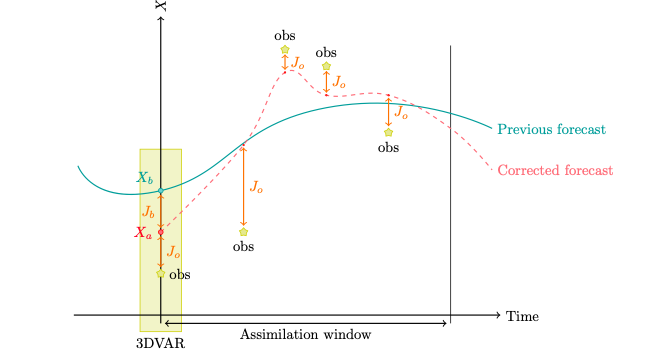
\includegraphics[width=0.8\textwidth]{"images/schema_3D_Var.png"}
	\end{center}
\subsubsection{From 3DVar to BLUE}
\noindent We have are 3D-Var cost function:
$$J(x)=\frac{1}{2}\|x-x^b\|_B^2+\frac{1}{2}\|H(x)-y\|_{R}^2 $$
 Let us minimize J and compute the variation of $J(x)$ with respect to
a variation of $x$ :
$$\begin{aligned}
\delta J(x)=&\frac{1}{2}(\delta x)^TB^{-1}(x-x^b) \\
&+\frac{1}{2}(x-x^b)^TB^{-1}\delta x \\ &+\frac{1}{2}(-H(\delta x))^TR^{-1}(y-H(x)) \\
&+\frac{1}{2}(x^b-H(x))R^{-1}(-H(\delta x)) \\
=&(\delta x)^TB^{-1}(x-x^b)-(\delta x)^TH^TR^{-1}(y-H(x)) \\
=&(\delta x)^T \nabla J
\end{aligned}$$
The extremum condition is 
$$\nabla J=B^{-1}(x^*-x^b)-H^TR^{-1}(y-Hx^*)=0$$
so we will have:
$$x^*=x^b+(B^{-1}+H^TR^{-1}H)^{-1}H^TR^{-1}(y-Hx^b)$$
Grave to Sherman-Morrison-Woodbury identity,
$$K^*=(B^{-1}+H^TR^{-1}H)^{-1}H^TR^{-1}=BH^T(R+HBH^T)^{-1}$$
Therefore, we have that our solution $x$ of the minimization problem coincides with the BLUE optimal analysis $x^a$
\subsection{Ensemble Kalman Filter}
\noindent We have seen so far two methods to do data assimilation, these methods are valid only for linear systems, but the Lorenz system is non-linear, that's why we will introduce the Ensemble Kalman Filter method which works well for non-linear systems. The ENKF method consists in using the Kalman filter method in high dimension and replace P by a set of states $x_1,x_2,..,x_{m}$. So we can approximate the moments of the error by the moments of the sample.
The we have:
$$x_i^a=x_i^f+K[y-h(x_i^f)]$$
We can also define the Kalman gains: 
$$K=P^f H^T(HP^f H^T+R)^{-1}$$
To begin with we can estimate the
forecast error covariance matrix as:
$$P^f=\frac{1}{m-1}\sum_{i=1}^{m}(x_i^f-\bar{x}^f)(x_i^f-\bar{x}^f)^T~~with~~\bar{x}^f=\frac{1}{m}\sum_{i=1}^{m}x_i^f $$ 
We can factorized the forecast error covariance matrix by:
$$P^f=X_f X_f^T$$
where $X_f$ is an $n \times m$ matrix whose columns are the normalized anomalies or normalized perturbations,
$$[X_f]_i=\frac{x_i^f-\bar{x}^f}{\sqrt{m-1}}$$
In addition, we have:
$$
\bar{x}^a=\frac{1}{m}\sum_{i=1}^mx_i^a~~,~~~~[X_a]_i=\frac{x_i^a-\bar{x}^a}{\sqrt{m-1}} $$	

	\newpage

	\section{Conclusion}
	
	\noindent To conclude all this and to summarize everything, we had as main goal to implement a parallel time resolution method for the Lorenz system, and to realize the data assimilation using the EnKF method. But to achieve these goals we had to understand the Lorenz system and try to implement several numerical resolutions to find a solution. Afterwards, we have implemented the parareal method for the parallel time resolution of ODEs and have verified its convergence in a case where the analytical solution is known (in our case we have chosen the harmonic oscillator). We have then applied this method to the Lorenz system and we have noticed a speed up compared to the sequential execution with the fine time step, which shows that the method is efficient. And finally, for the data assimilation part, we had to understand the principles of methods such as the Kalman filter and 3DVAR. It was also important to understand the link between these two methods in order to understand the method to use in the case where the differential equation system is nonlinear and to implement the method using EnKF with FilterPy. We noticed that during the data assimilation the covariance matrices associated with the error of our states had a very large impact on the analyses. Changing one of these parameters or reversing the covariance matrix associated with the error of the observations with the one associated with the model could seriously change our final analysis. 
	
	\newpage
	
	\section*{Bibliography}
	\addcontentsline{toc}{section}{Bibliography}
	
	\printbibliography[heading=subbibintoc,keyword=ref,title={References}]
	
	\newpage
	
	\printbibliography[heading=subbibintoc,keyword=doc,title={Documentation}]
	
	\appendix
	
	\lstset{style=bash}

\section{Organisation of the repository}

	\begin{minipage}{0.65\linewidth}
		For the organisation of the repository, we created several directories (Figure \ref{tree}):
		\begin{enumerate}[label=\textbullet]
			\item \textbf{src :} In this directory there is all the source code of the project. We have a first \textit{python} subdirectory which contains the python codes for the data assimilation and parareal parts, these files were created during the M1 project. Then we have a second subdirectory \textit{cpp} which contains the C++ codes of the same 2 parts.
			\item \textbf{examples :} Here there are examples of how to use python and C++ codes.
			\item \textbf{tests :} In this directory there are python and C++ tests of the code. For python tests we will use the pytest tool and for C++ we will use ctest (see Appendix \ref{compile}).
			\item \textbf{docs :} This directory gathers all the files that are used to generate the documentation of the project (see Appendix \ref{doc}). The \textit{sphinx} and \textit{doxygen} directories enable respectively to document the python code and the C++ code (thanks to the sphinx~\cite{sphinx_doc} and doxygen~\cite{doxygen_doc} tools). The \textit{antora} directory contains some explanations of the project which are accessible online (the antora~\cite{antora_doc} tool was used). For example it explains : the differential equations concerned by this project, the data assimilation methods, the parareal method... The documentations generated by the previous tools are available directly in the GitHub repository via a Continuous Integration (CI) that has been set up (see Appendix \ref{ci}).
			The directories \textit{gantt}, \textit{meeting}, \textit{presentation} and \textit{report} contain all the latex files and images used for the presentations and reports requested in the context of the internship.
			\item \textbf{cmake/build :} The directory \textit{cmake} contains cmake configuration files which are used for the compilation of the C++ project (see Appendix \ref{compile}). The directory \textit{build} contains all the files generated by the compilation of the C++ code.
		\end{enumerate}
	\end{minipage} \qquad
	\begin{minipage}{0.33\linewidth}
		\begin{figure}[H]
			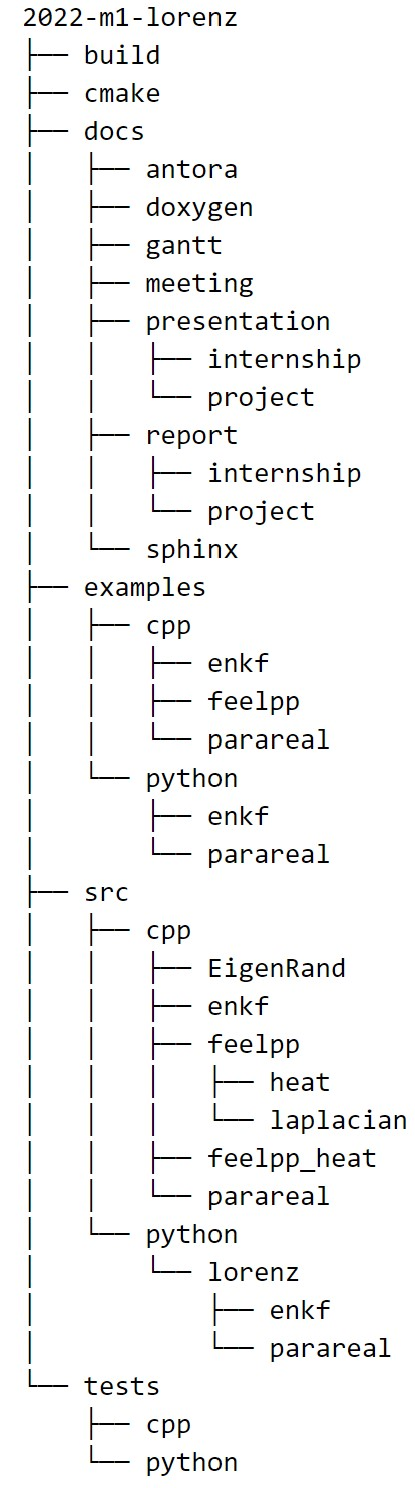
\includegraphics[width=\textwidth]{"images/appendix/tree.jpg"}
			\caption{Repository tree}
			\label{tree}
		\end{figure}
		%\lstinputlisting[language={},inputencoding=utf8]{tree.txt}
	\end{minipage}

\newpage

\section{Compile and test}
\label{compile}

	As explained in the previous section, the project includes both C++ and Python code. Let's see how to use these source codes :
	\begin{enumerate}[label=\textbullet]
		\item \textbf{Python :} \\
		Here all methods are grouped in a module called \textit{lorenz}. To execute the examples, we first need to add the path to the source code in the PYTHONPATH variable using the following command at the root of the project :
\begin{lstlisting}
		export PYTHONPATH=$PWD/src/python
\end{lstlisting}
		\fbox{ENKF ?} \\
		To run the examples for the parareal method with 2 processes, go to "examples/python/parareal" and then execute :
\begin{lstlisting}
		mkdir data_parareal
		mpirun -n 2 python3 examples_parareal.py [0,1,2]
\end{lstlisting}
		To run the tests we use the pytest tool. To do this, go to "tests/python" and run the following command :
\begin{lstlisting}
		pytest
\end{lstlisting}
		\item \textbf{C++ :} \\
		For the C++ code, we decided to write a CMake\footnote[1]{Minimum version required : 3.21} with presets~\cite{cmake_preset}.  A recurrent problem of CMake users is to share settings with other people for common ways of configuring a project. A solution to this is to define a "CMakePresets.json" file at the root of the project allowing to define different compilation modes. \\
		We defined 3 presets : \textit{default} is the default compilation mode, \textit{dbg} the mode to debug the code and \textit{doc} to generate the documentation (see Appendix \ref{doc}). \\
		These are the commands to configure and build in default mode :
\begin{lstlisting}
		cmake --preset default
		cmake --build --preset default
\end{lstlisting}
		The executables generated by the last command will then be stored in the "build/default/bin" directory. There you will find :
		\begin{itemize}[label=-]
			\item \textbf{enkf.e : } \fbox{ENKF ?}
			\item \textbf{parareal.e : } To run in parallel with 4 processes :
\begin{lstlisting}
		mpirun -n 4 ./build/default/bin/parareal.e
\end{lstlisting}
			This applies the parareal method to the Lorenz system with parameters defined in the code and displays the number of iterations of the method as well as the execution time. 
			\item \textbf{laplacian.e : } To run in sequential:
\begin{lstlisting}
		./build/default/bin/laplacian.e 
				--config-file <cfg_filename>
\end{lstlisting}
			To run in parallel with 4 processes:
\begin{lstlisting}
		mpirun -n 4 ./build/default/bin/laplacian.e 
				--config-file <cfg_filename>
\end{lstlisting}
			This allows to solve the Laplace equation from a given geometry by the finite element method by using Feel++~\cite{feelpp_laplacian}.
			\item \textbf{heat.e : } \\
			This solves in parallel the heat equation from a given geometry with the parareal method by using Feel++. \\
			We will place ourselves in the following test case. \\
			The spatial domain is partitioned into 2 sub-domains using the command :
\begin{lstlisting}
		feelpp_mesh_partitioner --dim=2 --part 2 
				--ifile <geo_filename> 
\end{lstlisting}
			We also partition the temporal domain into 2 sub-domains, which makes 2*2 processes for the fine integrator and 2 processes for the coarse integrator, so 6 processes in all. We can then run in parallel with 6 processes :
\begin{lstlisting}
		mpirun -np 6 ./build/default/bin/heat.e 
				--config-file <cfg_filename>
\end{lstlisting}		
		For more details see Section \ref{heat}.
		\end{itemize}
		For C++ tests, we use the ctest tool in the following way:
\begin{lstlisting}
		ctest --preset default
\end{lstlisting}
	\end{enumerate}

\newpage

\section{Documentation}
\label{doc}

\newpage

\section{Github actions}
\label{ci}	
	
\end{document}
